%% ------------------------------------------------------------------------- %%
\chapter{Conceitos}
\label{cap:conceitos}

Este capítulo apresenta, um a um, os conceitos mais elementares 
e tenta harmonizar a terminologia empregada no decorrer do texto.


%% ------------------------------------------------------------------------- %%
\section{\Gls{tectonic}}
\index{\gls{tectonic}}
\label{sec:02_tectonica}

A \gls{tectonic} é \glsdesc*{tectonic}.

Uma das principais evidências das transformações geológicas do planeta 
são os \glspl{equake}. A figura \ref{f:global_epicenters} \citep{lowman_jr_1998}
é um mapa global com a ocorrência geográfica dos tremores. Nele é possivel notar que 
os sismos não são distribuídos uniformemente pelo globo.

\begin{figure}[H]
   \centering
   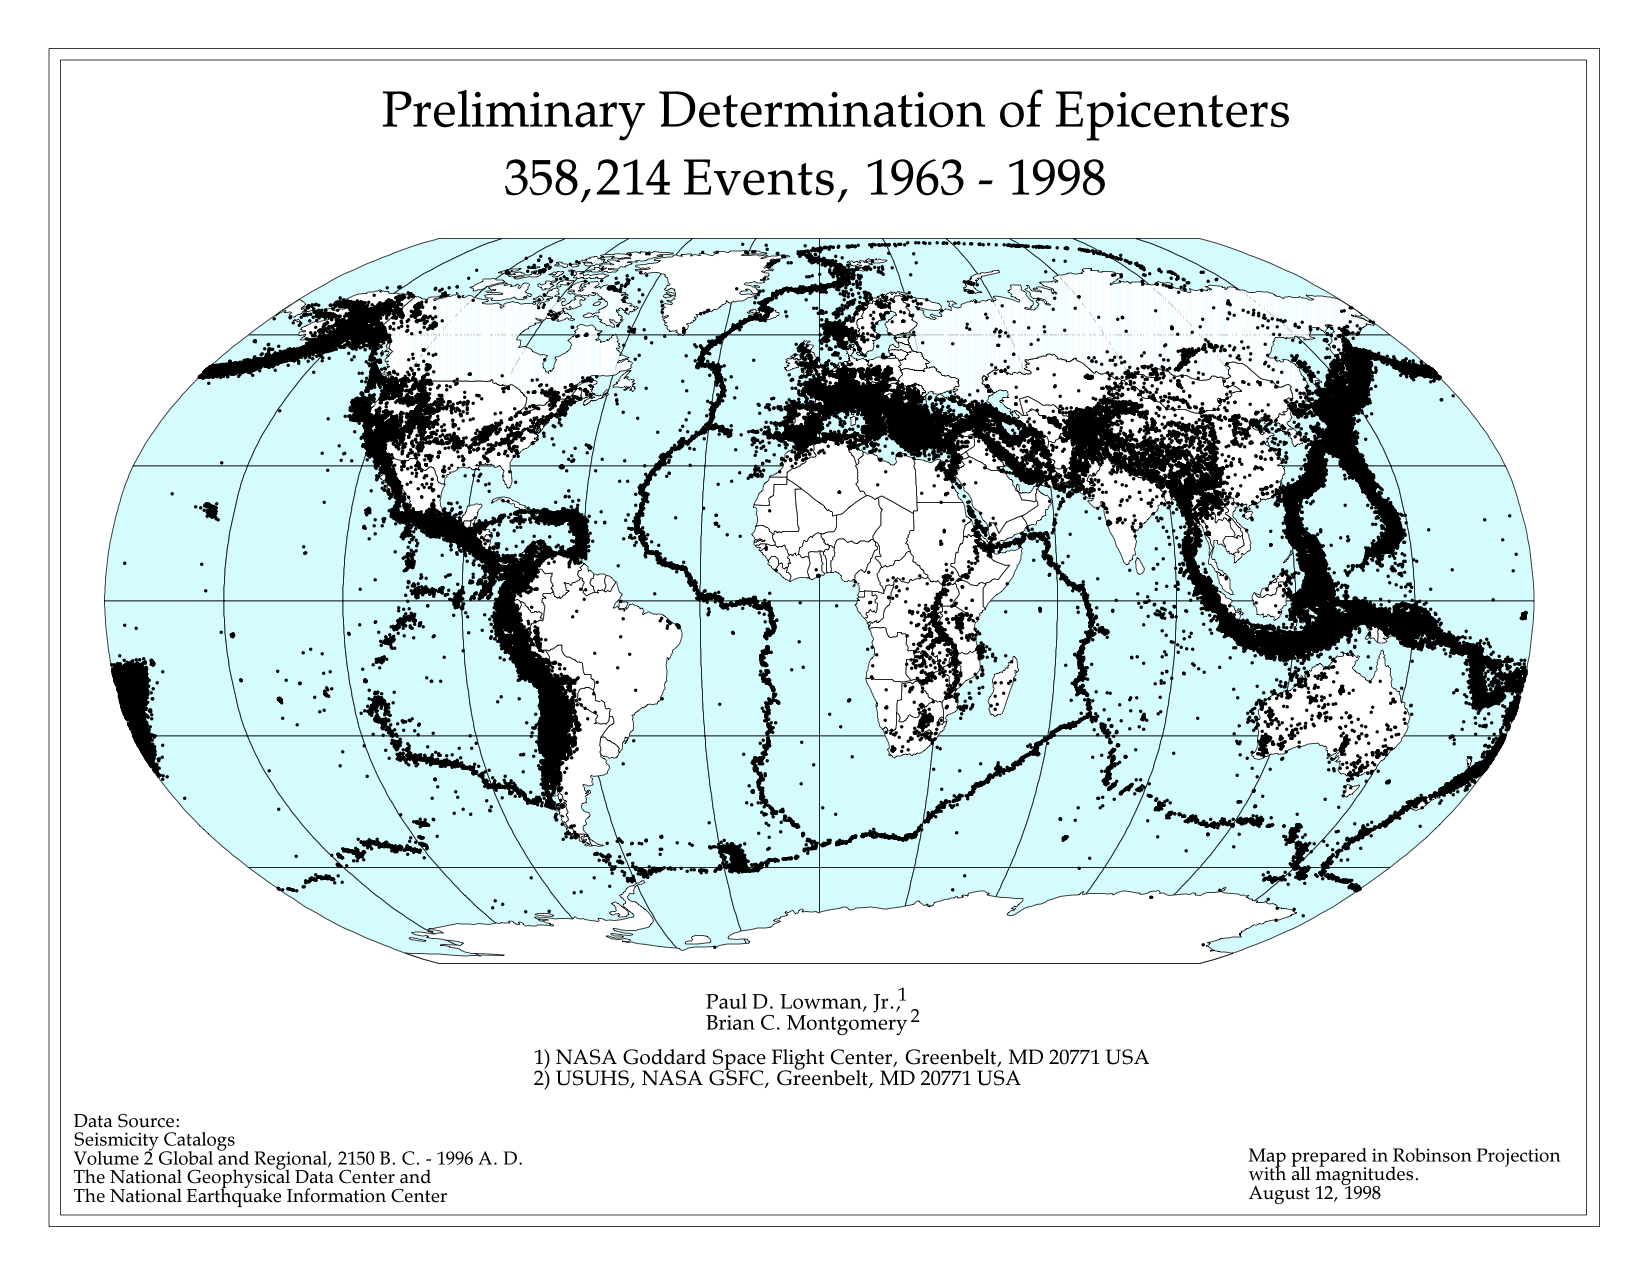
\includegraphics[width=0.80\textwidth]{global_pde_mag_all}
   \caption{Mapa Mundial de Epicentros} 
   \label{f:global_epicenters}
\end{figure}

O padrão apresentado pela \gls{seismic_activity} global foi essencial 
para o desenvolvimento posterior da \gls*{tectonic_plate_theory}.

%% ------------------------------------------------------------------------- %%
\subsection{\Gls{tectonic_plate_theory}}
\index{\Gls{tectonic}!\Gls{tectonic_plate_theory}}
\label{sec:02_placas}

A \gls*{tectonic_plate_theory}, desenvolvida na segunda metade do século XX,
cartografava na superfície do globo as \glspl{litho_plate}.


\begin{figure}[H]
   \centering
   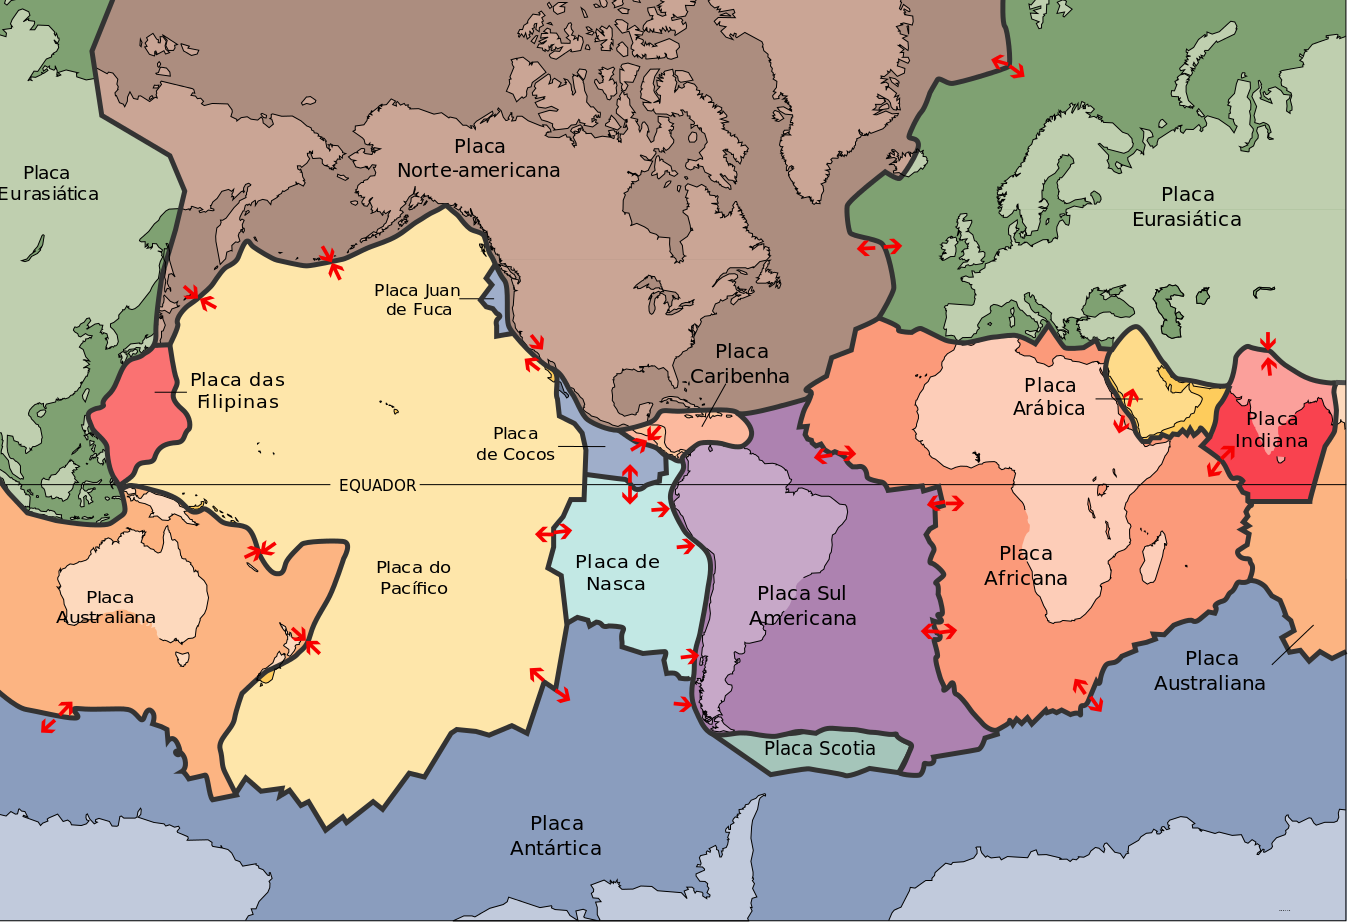
\includegraphics[width=0.80\textwidth]{litho_plates_overview}
   \caption[Cartografia das placas litosféricas]
   		   {Cartografia das placas litosféricas} 
   \label{f:plates_overview}
\end{figure} 
 
As \glspl{litho_plate}, como pode ser visto na figura \ref{f:plates_overview} \citep{usgs_plates_1996},
e o conceito de \gls{astenosphere} (\glsdesc{astenosphere}) 
surgem para conformar uma teoria capaz de explicar
uma série de fenômenos tectônicos observados e ainda não bem explicados naquela época. 


%% ------------------------------------------------------------------------- %%
\subsubsection{Bordas}
\index{\Gls{tectonic_plate_theory}!bordas}
\label{sec:02_bordas}

Nas bordas das \glspl{litho_plate} a tectônica é mais intensa
provocando uma enorme diversidade de fenômenos geológicos de acordo
com o tipo de interação. Algumas delas estão esquematizadas na 
figura \ref{f:plate_boundaries} \citet{vigil_1997}.

\begin{figure}[H]
   \centering
   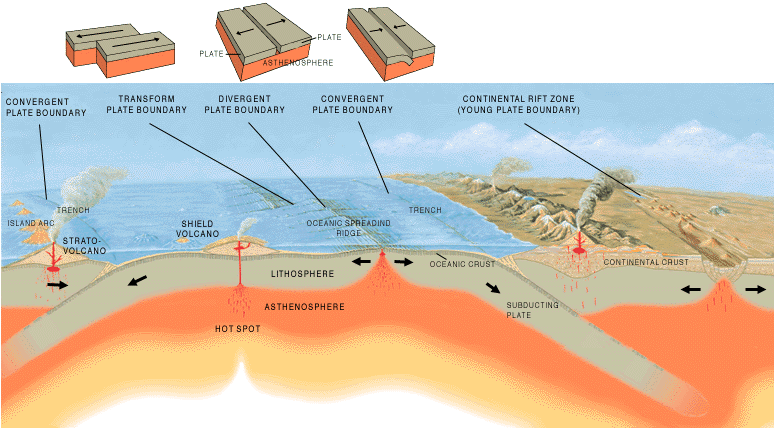
\includegraphics[width=0.95\textwidth]{plate_boundaries}
   \caption[Diferentes tipos de interações entre \glspl{litho_plate} em suas bordas]
   		   {Diferentes tipos de interações entre \glspl{litho_plate} em suas bordas} 
   \label{f:plate_boundaries}
\end{figure} 
 
Na figura \ref{f:plate_boundaries} estão ilustrados os diferentes tipos de interação 
entre as \glspl{litho_plate} nas suas bordas, que causam, como já se sabe, a maior
parte dos \glspl{equake} e vulcanismo.

Só na borda das placas é liberada cerca de 95\% da quantidade total da energia 
disseminada na forma de \glspl{equake} no globo.

%% ------------------------------------------------------------------------- %%
\subsubsection{Interior}
\index{\Gls{tectonic_plate_theory}!interior}
\label{sec:02_interior}

A dificuldade é explicar, com maior detalhe, porque e como são liberados os outros 
5\% do total de energia em \glspl{equake}, mais raros, no interior das \glspl{litho_plate}.

Não há pleno consenso nem um modelo geral para a explicação do mecanismo de ocorrência dos
sismos no interior das placas \citep{talwani_2014} embora sejam conhecidas diversas zonas sísmicas em regiões no
interior de placas que apresentam sismicidade importante com sismos cujas
magnitudes em alguns casos foram superior a 7, como em Nova Madrid, nos Estados Unidos 
e em locais da China e da Austrália para citar alguns outros.


%% ------------------------------------------------------------------------- %%
\subsection{Sismotectônica}
\index{\gls*{seismotectonic}}
\label{sec:sismotectonica}

A \gls{seismotectonic} é \glsdesc*{seismotectonic}. 

Na prática consiste por um lado, num esforço de compreensão dos
processos geológicos através da observação dos tremores e analogamente, compreender os tremores através da observação
de processos geológicos mensuráveis.  

É fácil notar a contribuição dessa disciplina para a análise de sismicidade e vice-versa.







\section{Probabilidade}
\index{probabilidade}
\label{sec:probabilidade}



\subsection{\Glsdesc{pdf}}
\index{\glsdesc{pdf}}
\label{sec:pdf}

A \gls{pdf} de uma \gls{va}  
descreve a probabilidade de que essa \gls{va} 
assuma, entre todas as realizações possíveis, uma em especial.

Seja $X$, uma \gls{va} unidimensional. A \gls{pdf}
$f_X(x)$ de $X$ é definida por

\begin{equation}
	P \left\{ X \in [x_0,x_1[\, \right\} = \int_{x_0}^{x_1}\!f_X(x)\,\mathrm{d}x, \; \forall x_0 \leq x_1 \in \mathbb{R}.
	\label{eq:pdf}
\end{equation}

Para que uma função possa assumir o papel de \gls{pdf} é necessário que ela
possua as seguites propriedades:
\begin{enumerate}[(i)]
	\item $f_X(x) \ge 0\;\forall x$  (a função $f_X$ deve ser sempre positiva), e
	\item $\int_{-\infty}^{+\infty} f_X(x) \mathrm{d}x = 1$ (e deve somar, sobre todos os valores possíveis, a unidade).
\end{enumerate}


\subsection{\Glsdesc{pmf}}
\index{\glsdesc{pmf}}
\label{sec:pmf}

Outro conceito importante e diretamente relacionado à \gls{pdf} é a
\gls{pmf}.

No caso da \gls{va} $X$, sua \gls{pmf} $F_X(x)$ é definida como

\begin{equation}
	P \left\{ X \leq x\right\} = F_X(x) = \int_{-\infty}^{x}\!f_X(u)\,\mathrm{d}u.
	\label{eq:pmf}
\end{equation}



\subsection{Histograma}
\index{histograma}
\label{sec:histogram}

Quando a \gls{pdf} de uma \gls{va} não é conhecida e se deseja estudar seu comportamento
é preciso estimá-la e para isso o histograma é uma das técnicas mais antigas e amplamente utilizadas.

O histograma divide o universo das observações, possíveis realizações $X_1, X_2,\cdots, X_n$
da \gls{va}, em compartimentos (\emph{bins}).

Dados uma origem arbitrária $x_0$ e uma largura $h$ de cada um, os compartimentos
são definidos como os intervalos $[x_0 + (j -1)h,\; x_0 + jh[$ 
com $j\in\mathbb{Z}$, um identificador para cada um deles. 

Considere um determinado intervalo $[-h/2, h/2[$. 
A probabilidade (\eqref{eq:pdf}) de que uma observação qualquer venha a pertencer a esse intervalo é

\begin{equation}
	P \left\{ X \in [-h/2,h/2[ \; \right\} = \int_{-h/2}^{h/2}\!f_X(x)\,\mathrm{d}x.
	\label{eq:hist01}
\end{equation}

E um estimador natural $\hat{f}_X$ para a densidade $f_X$ seria contar o número de observações

\begin{equation}
	P \left\{ X \in [-h/2,h/2[ \; \right\} \approx \frac{\# \left\{ X_i \in [-h/2,h/2[ \; \right\}}{n} =
	\int_{-h/2}^{h/2}\!\hat{f}_X(x)\,\mathrm{d}x ,
	\label{eq:hist02}
\end{equation}
de onde 
\begin{equation}
	\hat{f}_X(x) = \frac{\# \left\{ X_i \in [-h/2,h/2[ \; \right\}}{nh},
	\label{eq:hist_03}
\end{equation}
para todo $x \in [-h/2,h/2[$.

De modo geral, sejam $X_1, \cdots, X_n$ observações \gls{iid} da \gls{va} $X$ com densidade desconhecida $f$. 
Considere $N_I$ intervalos de comprimento $h$ e o conjunto de compartimentos $C_j = [x_0 + (j -1)h,\; x_0 + jh[,\;
j=1..N_I$.
Defina
\[
	I_A(x) := \begin{cases}
		1 & \text{se } x \in A \\
		0 & \text{caso contrário}
	\end{cases}
\] 
e 
\[	n_j := \sum_{i=1}^{n}I_{C_j}(X_i)\; \text{tal que} \;  \sum_{j=1}^{N_I}n_j = n. \]

Dessa forma a estimativa $\hat{f}$ parametrizada pela largura $h$ para a densidade $f$ seria
\begin{equation}
	\hat{f}(x \arrowvert\, h) = \frac{1}{nh} \sum_{j=1}^{N_I}n_jI_{C_j}(x)
	\label{eq:hist_04}
\end{equation}
para toda realização possível $x$ de $X$.






\section{Sismicidade}
\index{sismicidade}
\label{sec:sismicidade}

A sismicidade é a ocorrência dos tremores de terra. Como, quando, onde, de que tamanho?

É sabido que pequenos abalos são mais frequentes que os tremores de terra
muito grandes e catastróficos cujos registros são extremamente raros.

A figura \ref{f:m9} apresenta os sismos de magnitude acima de nove conhecidos.

\begin{figure}[H]
   \centering
   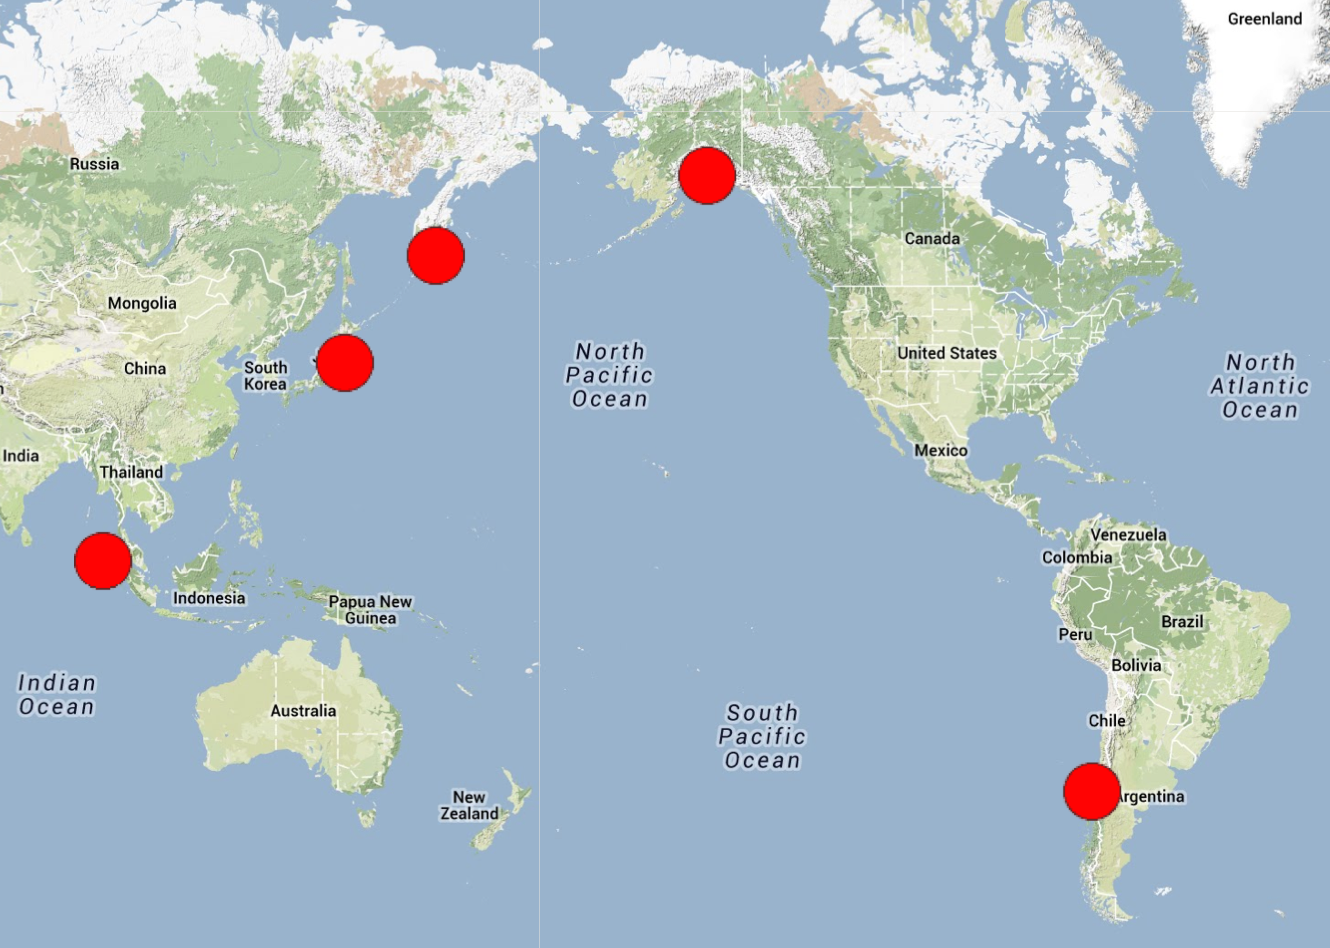
\includegraphics[width=0.5\textwidth]{M9}
   \caption[Sismos com magnitude acima de 9,0.]
   		   {Sismos com magnitude acima de 9,0. Fonte: \gls{isc}} 
   \label{f:m9}
\end{figure} 


Tremores de terra, abalos, \glspl{equake}, sismos são a ocorrência de
fenômenos geológicos de ruptura, instantânea, por certo mecanismo, de certa dimensão, na
crosta terrestre.

\subsection{Ocorrência}
\index{\gls{equake}!ocorrência}
\label{sec:ocorrencia}
 
Os tremores acontecem por uma ruptura geológica (figura \ref{f:rupture}) 
num instante \gls{sym:t}, num lugar \gls{sym:r} e cada um
com sua magnitude \gls{sym:m} associada.

\begin{figure}[H]
   \centering
   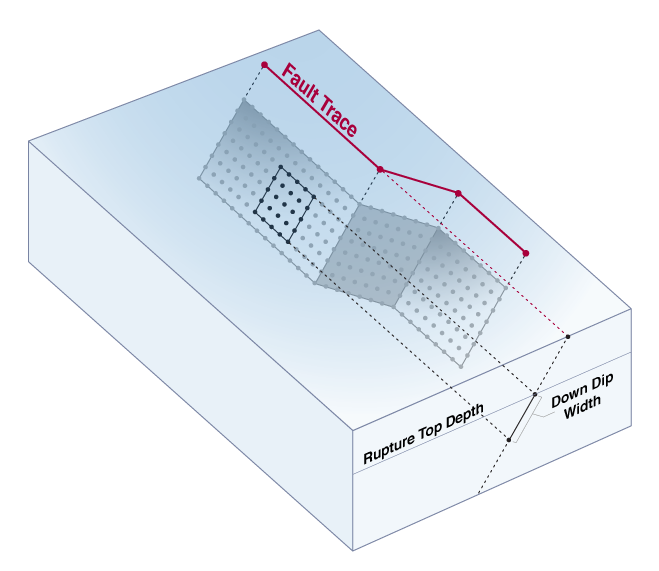
\includegraphics[width=0.50\textwidth]{rupture}
   \caption[Ilustração da área de ruptura em um falhamento geológico]
   		   {Ilustração da área de ruptura em um falhamento geológico\footnotemark} 
   \label{f:rupture}
\end{figure} 
\footnotetext{\citet{opensha_team_2010}}


O local em que se iniciou a ruptura que deu origem ao tremor é um \gls{hypocenter},
enquanto sua projeção na superfície, desconsiderando-se a profundidade, é o \gls{epicenter}.


\subsection[Magnitude]{Magnitude (da ruptura)}
\index{magnitude}
\label{sec:magnitude}

A magnitude de um tremor de terra é um valor medido numa escala que versa sobre a energia liberada pelo sismo.
Essa energia é proporcional à área rompida e ao deslocamento geológico relativo entre os blocos de rocha na superficie
de ruptura.

O desenvolvimento experimental de escalas de magnitude, para medir o tamanho dos tremores,
é marcado pelo trabalho do sismólogo Charles \citet{richter_1935}. Existem, entretanto, 
uma série de diferentes escalas de magnitude, baseadas em diversos tipos de medidas. 

A escolha de qual usar fica a critério
de cada sismólogo (ou analista) e de cada rede sismográfica. 
Geralmente usam escalas diferentes
para avaliar a magnitude dos tremores ou até mesmo divulgam mais de um tipo de magnitude para
um mesmo evento.

As escalas são calibradas para fornecerem valores similares, de acordo com
o intervalo de utilidade para o qual foram desenvolvidas, mas apresentam diferenças consideráveis para um mesmo evento.
Isso pode comprometer as análises estatísticas baseadas em um catálogo 
cujas magnitudes não tenham sido calculadas de maneira uniforme.


\subsubsection{Magnitude Richter}
\index{magnitude!Richter}
\label{sec:magnitude_richter}

As escalas de magnitude mais comuns são as que derivam da definição de \citet{richter_1935}
fundada na relação empírica entre o logarítmo da amplitude do registro das ondas sísmicas e a distância onde foram
registradas. Em 1935 Richter notou a seguinte proporcionalidade

\begin{equation}
	\gls{eqn:richter},
	\label{eq:richter}
\end{equation}
\glsdesc*{eqn:richter}.


A amplitude máxima de sua
escala foi definida pela amplitude máxima observada em um sismômetro Wood-Anderson, com período de 0.8s, registrando a 100km 
do tremor.

Algumas correções poderiam ser cogitadas, principalmente pelo fato da escala estar intimamente 
relacionada a um determinado equipamento, hoje obsoleto, e porque sismos locais (a menos de 100km) têm sua magnitude
melhor calculada usando frequências mais altas que as registráveis pelo sismômetro da época.


Outras escalas foram desenvolvidas a partir da medida da amplitude máxima de determinadas fases 
de diferentes tipos de onda sísmica e apresentam bons resultados para a maior parte dos sismos, 
mas não refletem, com precisão, 
o tamanho dos maiores e mais destrutivos eventos, com magnitude acima de 7 ou 8 porque geralmente saturam.


\subsubsection{Magnitude de Momento Sísmico }
\index{magnitude!momento sísmico}
\label{sec:momento_sismico}

O evento de natureza sismológica ocorre num
instante \gls{sym:t} liberando uma certa quantidade de energia na forma de \glsdesc{sym:M_0}
\gls{sym:M_0}. A \glsdesc{sym:MW} \gls{sym:MW} desse evento é proporcional ao logarítmo dessa energia 
\gls{sym:M_0}.

O \glsdesc{sym:M_0} é apresentado na equação \eqref{eq:M_0}:

\begin{equation}
	\gls{eqn:M_0}
	\label{eq:M_0}
\end{equation}
\glsdesc*{eqn:M_0}.

O momento sísmico é estimado geralmente pela inversão duplamente acoplada de um tensor de momento aos registros em 
forma de onda do movimento do chão causado pelo terremoto. Ou, em casos de tremores muito bem registrados, ele pode
ser estimado a partir de algum modelo numérico para a ruptura.

A \glsdesc{sym:MW} \gls{sym:MW} \citep{hanks_1979} é baseada no 
logarítmo do \glsdesc{sym:M_0} \gls{sym:M_0}, e não se satura no caso de grandes eventos. 
Sua definição é dada pela equação \eqref{eq:M_W} 

\begin{equation}
	\gls{eqn:M_W}
	\label{eq:M_W}
\end{equation}
\glsdesc*{eqn:M_W}.


\subsubsection{Intensidade Macrossísmica}
\index{instensidade macrossísmica}
\label{sec:intensidade}

A intensidade macrossísmica é uma escala para medir, não a energia proporcional
à ruptura que originou o tremor de terra, mas para retratar a percepção humana, e os efeitos sobre
construções e objetos, do movimento do chão onde quer este tenha produzido seus efeitos.

Uma das mais difundidas é a escala Modificada de Mercalli \citep{richter_1958} apresentada em sua versão simplificada 
na tabela \ref{tab:mercalli}:

\begin{table}[H]
\begin{center}
\begin{scriptsize}
\noindent\begin{tabular}{c|c|p{12cm}}
\hline
Categoria  	& Sensação & Efeitos \\
\hline
I 			&	Imperceptível 	&	Não sentido. Apenas registado pelos sismógrafos.
\\II 		&	Muito fraco 	&	Sentido por um muito reduzido número de pessoas em 
								repouso, em especial pelas que habitam em andares
								elevados.
\\III 		&	Fraco 			&	Sentido por um pequeno número de pessoas. Bem sentido nos andares elevados.
\\IV 		&	Moderado 		&	Sentido dentro das habitações, podendo despertar do sono um pequeno número de pessoas. 
								Nota-se a vibração de
								portas e janelas e das loiças dentro dos armários.
\\V 		&	Forte 			&	Praticamente sentido por toda a população, fazendo acordar muita gente. 
								Há queda de alguns objectos menos estáveis e param os pêndulos dos relógios. 
								Abrem-se pequenas fendas nos estuques das paredes.
\\VI 		&	Bastante forte 	&	Provoca início de pânico nas populações. Produzem-se leves danos nas habitações, 
								caindo algumas chaminés. O mobiliário menos pesado é deslocado.
\\VII 		&	Muito forte 	&	Caem muitas chaminés. Há estragos limitados em edifícios de boa construção, 
								mas importantes e generalizados nas construções mais frágeis. 
								Facilmente perceptível pelos condutores de veículos automóveis em trânsito. 
								Desencadeia pânico geral nas populações.
\\VIII 		&	Ruinoso  		&	Danos acentuados em construções sólidas. Os edifícios de muito boa construção 
								sofrem alguns danos. Caem campanários e chaminés de fábricas.
\\IX 		&	Desastroso 		&	Desmoronamento de alguns edifícios. Há danos consideráveis em construções muito sólidas.
\\X 		&	Destruidor 		&	Abrem-se fendas no solo. Há cortes nas canalizações, torção nas vias de caminho 
								de ferro e empolamentos e fissuração nas estradas.
\\XI 		&	Catastrófico 	&	Destruição da quase totalidade dos edifícios, mesmo os mais sólidos. 
								Caem pontes, diques e barragens. Destruição das redes de canalização e das vias de comunicação. 
								Formam-se grandes fendas no terreno, acompanhadas de desligamento. Há grandes escorregamentos de terrenos.
\\XII 		&	Cataclismo 		&	Destruição total. Modificação da topografia. Nunca foi presenciado no período histórico. \\
\hline
\end{tabular}
\caption{Escala simplificada de intensidade sísmica, 
modificada em 1956 derivada da escala original de Giuseppe Mercalli de 1902.}
\label{tab:mercalli}
\end{scriptsize}
\end{center}
\end{table}

Existem estudos \citep{bakun_1999} que propõem a inferência sobre o tamanho da ruptura, e sua
magnitude, a partir de observações macrossísmicas, ou dos efeitos relatados pela escala de intenside, georreferenciados.


%% ------------------------------------------------------------------------- %%
\subsection{Catálogos}
\index{catálogos}
\label{sec:catalogos}

Os catálogos podem ser vistos como uma coleção de parâmetros sobre os tremores. 
Podem ser classificados em três categorias \citep{woessner_2010} enumeradas a seguir:

\begin{itemize}\setlength{\itemsep}{0em}
	\item Pré-históricos: baseados na coleta de dados feitas por 
	geólogos estruturais em trincheiras ou campos de subsidência. Podem conter registros de tremores que ocorreram 
	há milhares de anos.
	\item Históricos: catálogos formados a partir de relatos históricos e inferência de valores de intensidade
	(seção \ref{sec:intensidade}), de análises de forma de onda com instrumentos antigos (registros em papel), eventualmente
	digitalizados.
	Cobrem o período das primeiras descrições humanas até os catálogos intrumentais.
	\item Instrumentais: são os catálogos de sismicidade definidos por dados produzidos por uma rede sismográfica bem estabelecida
	 gerando localizações continuamente (que começam a existir a partir de 1960).
\end{itemize} 

Os catálogos instrumentais são uma listagem onde se epera encontrar, para cada evento, as
seguintes informações:

\begin{itemize}\setlength{\itemsep}{0em}
	\item algum identificador,
	\item a localização (\gls{hypocenter}) do evento (longitude, latitude, profundidade) em algum sistema de referência,
	\item o tempo de origem (data e hora) com precisão de pelo menos décimos de segundo e
	\item uma ou várias informações de \glsdesc{sym:m}.
\end{itemize} 

Adicionalmente, embora não seja muito frequente, podem ser fornecidas informações adicionais obtidas pela análise das
formas de onda, como:

\begin{itemize}\setlength{\itemsep}{0em}
	\item incertezas sobre as magnitudes,
	\item incertezas sobre a localização (erro padrão, elipses de erro, cobertura dos sismogramas em diversas distâncias, cobertura
	dos sismogramas em vários ângulos azimutais, acurácia do modelo de velocidades utilizado, para enumerar alguns),
	\item intensidade máxima,
	\item intensidade no epicentro,
	\item número de, e as vezes as próprias, informações usadas para a determinação do hipocentro e hora de origem,
	\item sobre o mecanismo (alinhamento, mergulho e sentido do deslocamento na falha geológica) focal, entre outras.
\end{itemize} 

É importante salientar \citep{woessner_2010} que cada um dos parâmetros determinados é fruto de uma série de decisões
e etapas de processamento. Começam pela escolha dos sismômetros e pelos locais onde serão instalados para registrar as
formas de onda. Sinais acima do nível de ruído são associados à chegadas de fases quando registradas em mais de uma estação. 
A localização e o tempo de origem são determinados juntando-se os tempos de chegadas das fases a um modelo de velocidade
das ondas ao longo de camadas da crosta (ao qual a localização é extremamente dependente). As magnitudes, por fim, são
computadas a partir das amplitudes e/ou da duração do sinal, dependendo profundamente da calibração dos instrumentos.



\subsection{\glsdesc{mfd}}
\index{MFD}
\label{sec:mfd}

Observa-se que os sismos menores são muito mais frequentes.
Entretanto, os maiores e mais raros são os que trazem a maior ameaça e os que causam as maiores perdas.
Em virtude disso, uma análise conveniente seria explorar como se distribuem as magnitudes.

\subsubsection{\glsdesc*{mfd} (\gls{mfd}) de Gutenberg-Richter}
\index{Gutenberg-Richter MFD}
\label{sec:grmfd}

\citet{gutenberg_1944} observaram empiricamente que a distribuição da frequência de ocorrência dos tremores e
das magnitudes seguiam uma distribuição (de Pareto) cuja versão clássica é apresentada na equação \eqref{eq:gr_mfd} a
seguir:

\begin{equation}
	\gls{eqn:gr_mfd}
	\label{eq:gr_mfd}
\end{equation}
\glsdesc*{eqn:gr_mfd}.

Com uma simples transformação de variáveis ($\alpha = 10^a$ e $\beta = b\ln{10}$), observa-se que o número de sismos que ocorrem 
com magnitudes dentro de um pequeno intervalo $[m, m+\mathrm{d}m]$ é

\begin{equation}
	\begin{split}
		\gls{sym:N_m} &= 10^{\gls{sym:a} - \gls{sym:b}\gls{sym:m}} \\
					  &= \alpha e^{-\beta m}
	\end{split}
	\label{eq:gr_exp}
\end{equation}

A distribuição cumulativa, ou seja, o número de eventos com magnitude maior que um certo valor $m_{min}$, é apresentada
na equação \eqref{eq:gr_cum}:

\begin{equation}
	\begin{split}
		N(m > m_{min}) &= \alpha \int\limits_{m_{min}}^{\infty}e^{-\beta m}\mathrm{d}m \\
					   &= \frac{\alpha}{\beta} e^{-\beta m} \\
					   &= \alpha_{cum} e^{-\beta m}.
	\end{split}
	\label{eq:gr_cum}
\end{equation}
onde $\alpha_{cum} = \alpha / \beta $ é o valor cumulativo da atividade sísmica.


Entretanto, a distribuição clássica de \gls{gr} não impunha restrições sobre um limite inferior $m_{min}$ 
ou superior $m_{max}$ à validade da distribuição.



\subsubsection{MFD Truncada}
\index{MFD Truncada}
\label{sec:TMFD}

Variações da distribuição clássica de \gls{gr} foram propostas em vista de melhor representar as MFD estudadas à partir de
catálogos de diversas regiões.

A equação \eqref{eq:gr_max} versão incremental truncada com um limite superior $m_{max}$:

\begin{equation}
		\gls*{sym:N_m} = \frac{e^{-\beta m}}{1 -e^{-\beta m_{max}} }, m \leq m_{max}
	\label{eq:gr_max}
\end{equation}

Na equação \eqref{eq:gr_dtr} versão incremental duplamente truncada com um limite inferior $m_{min}$ e superior $m_{max}$ :

\begin{equation}
		\gls*{sym:N_m} = \frac{e^{-\beta (m - m_{min})}}{1 -e^{-\beta (m_{max} - m_{min}) } } , m_{min} \leq m \leq m_{max}
	\label{eq:gr_dtr}
\end{equation}

A figura \ref{f:mfd} ilustra essas distribuições.

\subsubsection{MFD Limitada}
\index{MFD Limitada}
\label{sec:BMFD}

Outra possibilidade, é limitar suavemente a parte final da curva (ver figura \ref{f:mfd}). A equação \eqref{eq:gr_bounded} apresenta
a distribuição:

\begin{equation}
		\gls*{sym:N_m} = \alpha [ e^{-\beta (m - m_{min})} - e^{-\beta (m_{max} - m_{min}) } ], m_{min} \leq m \leq m_{max}
	\label{eq:gr_bounded}
\end{equation}


\subsubsection{MFD com decaimento exponencial}
\index{MFD com decaimento exponencial}
\label{sec:KMFD}

Yan Kagan \citep{kagan_2002} propôs uma distribuição de magnitude mais adequada e acoplada à energia liberada pelos sismos, que
pode ser descrita como na equação \eqref{eq:gr_tapered}:

\begin{equation}\ensuremath{
		\gls*{sym:N_m} = [\gls*{sym:beta_p} + \frac{m}{m_{min}}]
				m_{min}^{\gls*{sym:beta_p}}
				\gls*{sym:m_corner}^{-1 -\gls*{sym:beta_p}}
				e^{\frac{m_{min} - m}{\gls*{sym:m_corner}}}, 
				m_{min} \leq m < \infty
		}
	\label{eq:gr_tapered}
\end{equation}
onde \glsdesc*{sym:beta_p} e \gls*{sym:m_corner} \glsdesc*{sym:m_corner}

\begin{figure}[H]
   \centering
   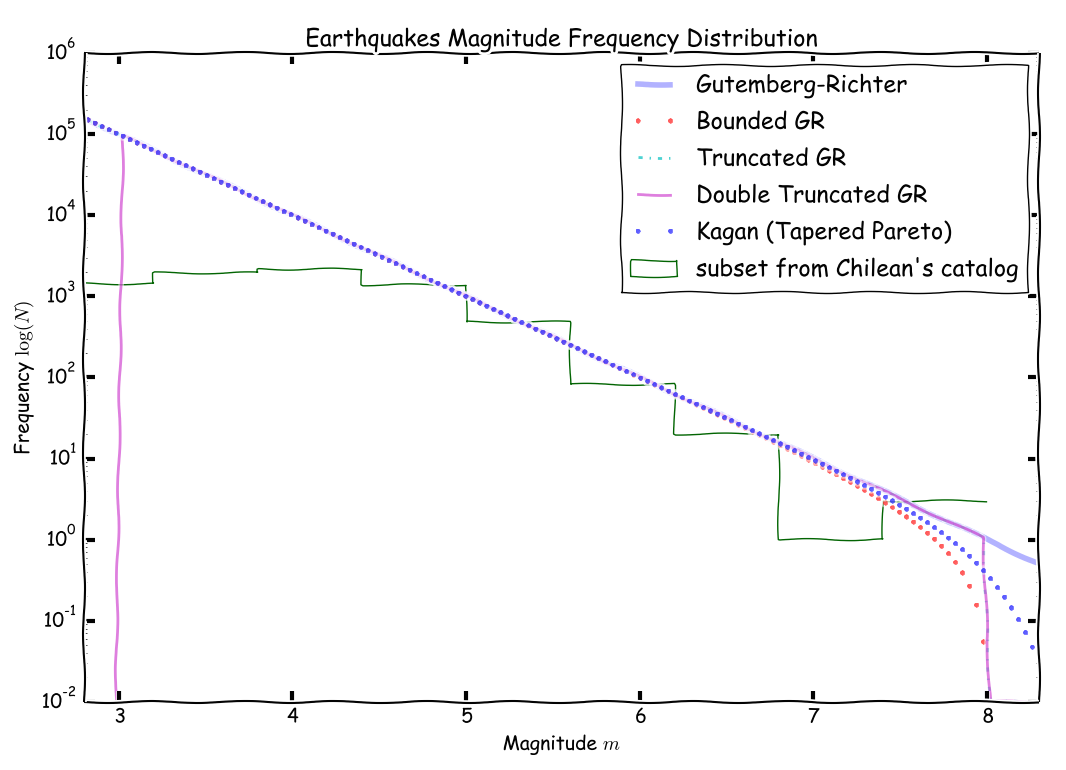
\includegraphics[width=0.95\textwidth]{mfd}
   \caption[Distribuições de frequência e magnitude]
   		   {Distribuições de frequência e magnitude} 
   \label{f:mfd}
\end{figure} 

A figura \ref{f:mfd} apresenta um comparativo de algumas distribuições. Para ilustração, 
há também na figura um histograma de um catálogo de
uma pequena região do norte do Chile, onde se pode observar que tanto a porção inferior (em torno de $m=5$), como a porção
posterior ($m > 7$) do histograma não seguem perfeitamente a distribuição. Há essencialmente duas zonas críticas em que é preciso
estar atento à física do problema:
(i) na parte inferior, muitos sismos de magnitude pequena não são registrados, seja por não terem energia suficiente
para sensibilizar um conjunto razoável de estações que permitam determinar suas localizações, seja porque o número de
estações é insuficiente na região onde os pequenos tremores ocorrem; (ii) a parte superior, por sua vez, é crítica
por se acoplar diretamente aos limites físicos do tamanho da maior ruptura possível, relacionada diretamente ao limite de liberação de energia na forma de momento sísmico $M_0$.

Nas distribuições de magnitude e frequência é importante que se possa reconhecer claramente alguns parâmetros
fundamentais.

\subsection{Valor-b}
\index{valor-b}
\label{sec:b_value}

O \emph{valor-b} foi apresentado na seção \ref{sec:grmfd} como sendo a inclinação da reta que representa a parte linear
descrescente da distribuição. Representa a proporção entre sismos pequenos e catastróficos que uma determinada fonte
sísmica é capaz de produzir (figura \ref{f:occurrence}).

\begin{figure}[H]
   \centering
   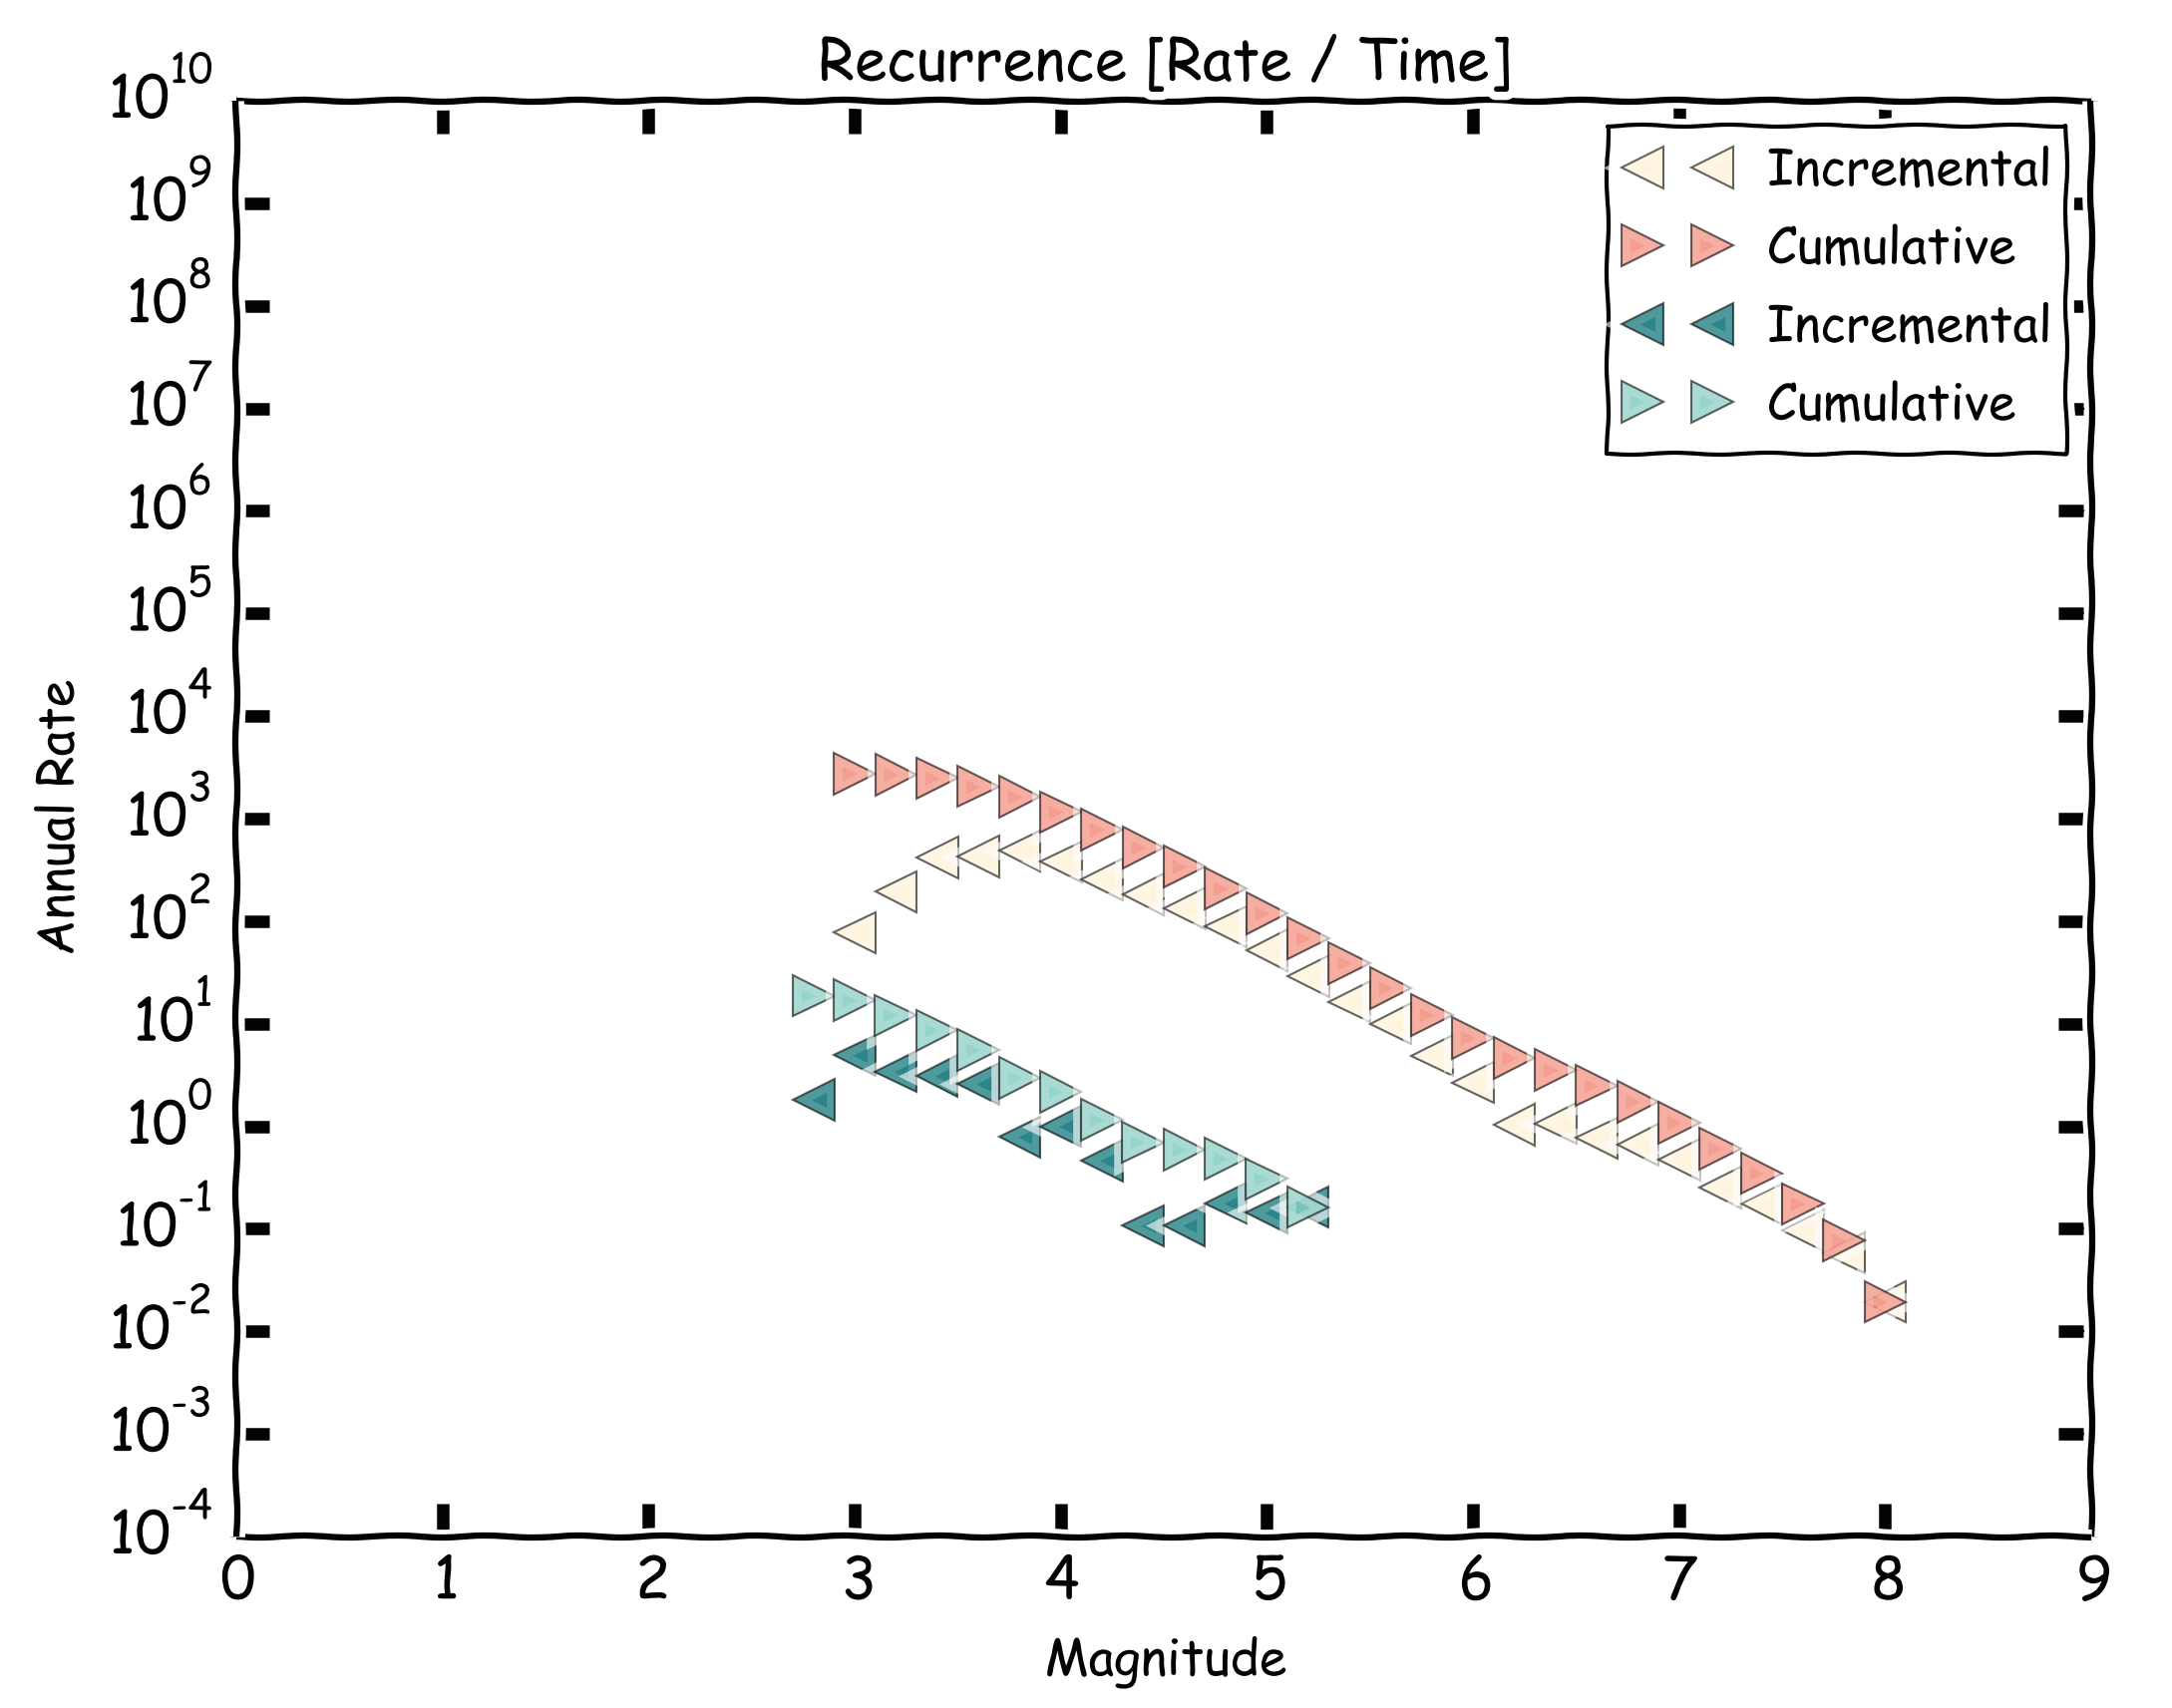
\includegraphics[width=0.95\textwidth]{occurrence}
   \caption[Distribuição incremental e cumulativa de frequência e magnitude dos sismos presentes no catálogo ISC-GEM
   para a América do Sul unido com o \gls{bsb2013}]
   {Distribuição incremental e cumulativa de frequência e magnitude dos sismos presentes no catálogo ISC-GEM
   para a América do Sul unido com o \gls{bsb2013}} 
   \label{f:occurrence}
\end{figure} 
%\footnotetext{\citet{img_opensha_rupture}}
 



\subsection{Taxa de Sismicidade}
\index{taxa de sismicidade}
\label{sec:seismic_rate}

A taxa de sismicidade é a medida da ocorrência dos tremores por uma determinada unidade de tempo (geralmente anos).
Representa para cada magnitude, a frequência média de ocorrência de sismos.

\subsection{Valor-a}
\index{valor-a}
\label{sec:a_value}

O \emph{valor-a} é a interseção da \gls{mfd} no eixo das frequências e representa o nível geral de sismos
que as fontes observadas pelo catálogo são capazes de produzir.

Costuma ser confundido pela forma de representação adotadas para a distribuição (incremental e/ou
cumulativa) e pelos truncamentos onde por vezes se apresenta o valor-a como a taxa de sismicidade da 
magnitude mínima ou de completude do catálogo.

No presente trabalho o \emph{valor-a} significará sempre o da distribuição cumulativa de sismos por unidade de
tempo com magnitudes positivas.

\subsection{Magnitude de Completude $M_c$}
\index{magnitude de completude}
\label{sec:completeness}

A magnitude de completude é o valor mínimo para o qual a distribuição é capaz de observar completamente o conjunto
de sismos. Em outras palavras representa o limite de observação completa do catálogo.

Sua identificação é bem simples quando se observa a distribuição incremental de magnitudes. É facilmente notado o valor
de magnitude na porção inferior na qual o número de sismos registrados começa a divergir da tendência geral da
distribuição.

Seu mapeamento é importante uma vez que os métodos de ajuste e determinação dos parâmetros da distribuição baseados na
máxima verossimilhança \citep{aki_1965, weichert_1980} dependem fundamentalmente desse valor mínimo.


\section{Risco Sísmico}
\index{Risco Sísmico}
\label{sec:risco_sismico}

A redução do risco sísmico é um problema complexo que envolve geralmente muitas pessoas, informações, decisões e ações.

A palavra risco, ao pé da letra, significa a exposição à possibilidade de injúria ou perda. E geralmente é usada como
sinônimo de ameaça. Na literatura acerca do tema risco, inclusive, as palavras risco e ameaça são usadas com certa
confusão.

No glossário da \gls{eeri} (EERI Committee on Seismic Risk, 1984) a definição de risco sísmico é a probabilidade de
que perdas sociais ou econômicas aconteçam como decorrência de tremores por superarem limiares estabelecidos para
determinado local ou região durante um certo período de exposição.

A ameaça sísmica, por outro lado, é qualquer fenômeno físico (oscilação, falhamento) associado à terremotos que possam
produzir efeitos adversos às atividades humanas. Na prática são avaliados por dadas probabilidades de ocorrência.

Pode-se deduzir que o risco sísmico é então uma combinação da ameaça sísmica com outros fatores:

\begin{equation}
		\text{Risco Sísmico} = \text{Ameaça Sísmica} \ast \text{Vulnerabilidade} \ast \text{Valor Exposto},
	\label{eq:risk}
\end{equation}

onde a vulnerabilidade é a quantidade de danos induzidos por um dado grau de ameaça e expressa como uma fração do
valor exposto ao dano e varia de acordo com o modelo proposto.

Frequentemente, o fator vulnerabilidade advém das análises das (ii) respostas das estruturas edificadas ao espectro de
acelerações produzidos pela (i) provável ameaça sísmica e da análise de possíveis (iii) danos estruturais à edificação.

A decisão de alterar ou não o desenho estrutural das edificações é feito a partir da análise dos (iv) prejuízos
(quantidade de moeda, mortes, tempo inoperante) causados caso as estruturas sejam danificadas conforme as análises anteriores.


\section{Ameaça Sísmica}
\index{ameaça sísmica}
\label{sec:ameaca_sismica}

A ameaça sísmica poderia ser definida de modo geral como a possibilidade de ocorrerem efeitos potencialmente destrutivos
de um terremoto em uma particular localização. Com exceção de \textit{tsunamis} ou falhamentos geológicos superficiais,
todos os efeitos destrutivos de um tremor de terra estão diretamente relacionados ao movimento do chão induzido pela
passagem das ondas sísmicas. Existem, entretanto diferenças de abordagem para a avaliação da ameaça sísmica.

A \glsdesc{psha} foi introduzida por \citet{cornell_1968}, aprimorada por \citet{mcguire_1976} e se tornou técnica mais
amplamente utilizada para a avaliação da ameaça sísmica. Também é possível fazer essa avaliação deterministicamente,
através de cenários definidos pelo espectro de movimento forte do chão que pode ser causado pela ocorrência de um
determinado tremor de terra em certa localização e de certa magnitude. O possível espectro de movimento no local de
interesse é avaliado através de relações de atenuação ou \glspl{gmpe}.

Os mecanismos da \gls{psha} \citep{bazzurro_1999, abrahamson_2006} são menos óbvios do que os da \gls{dsha}
\citep{reiter_1991, kramer_1996}, e em essência significam identificar todos os possíveis tremores que podem afetar o local de interesse,
incluíndo todas as possíveis combinações de distâncias e caracterizar a frequência de ocorrência das diferentes magnitudes através de relações de recorrência. As equações de
atenuação são utilizadas para calcular os parâmetros do movimento do chão no local de interesse devido a esses tremores
e consequentemente a taxa com que diferentes níveis de movimento do chão ocorram no local de interesse. 

Seus resultados também apresentam certa distinção. Se por um lado a \gls{psha} traz consigo o aspecto
temporal, ou a taxa com que diferentes níveis de aceleração excederão determinado limiar em determinado local de interesse,
por outro, a \gls{dsha} apresenta o movimento do chão esperado quando ocorra determinado evento de controle.


\section{Projeção da Ocorrência de Rupturas}
\index{projeção de ocorrência de rupturas}
\label{sec:projecao}

As projeções (\textit{forecasting}) são feitas para se estimar a ocorrência de futuros tremores 
\citep{kagan_2000,marzocchi_2011}, principalmente dos maiores, com grandes chances de provocar perdas.

Nas de curto prazo, estimam-se os próximos tremores
numa escala de dias ou horas considerando uma taxa de sismicidade variável 
com o tempo como no caso dos pré e pós-abalos, ou de quando 
acontece um enxame sísmico, período de maior atividade numa região.
Sua principal aplicação é auxiliar a tomada de decisões de curto período, 
como evacuação de edifícios.

Nas de longo prazo, foco desse texto, a principal consideração feita é de que a 
\gls{seismic_rate} não varie ao longo do tempo, servindo para estimar as acelerações 
provocadas por tremores, mesmo que possam ocorrer
muito raramente, de grandes proporções. 

São geralmente aplicadas quando
se deseja saber o nível de segurança e resistência estrutural que devem ser impostos 
às edificações em geral, ou quando se deseja estimar o valor de um contrato de resseguro
de algum outro grande investimento.


\section{Análise Probabilística de Ameaça Sísmica }
\index{PSHA, Análise Probabilística de Ameaça Sísmica}
\label{sec:psha}


Na \gls{psha} são considerados todos os possíveis tremores, as rupturas que os originaram e os movimentos do chão
resultantes conjuntamente com suas probabilidades de ocorrência associadas de modo a encontrar o nível de movimento do
chão que será excedido, numa janela de tempo, com uma pré-definida baixa tolerância \citep{baker_2008-1}.

Uma das formas de se enxergar o resultado de uma análise de ameaça sísmica
é como uma estimativa da pequena probabilidade $\xi$, em uma janela de tempo dada, 
com que determinada medida de intensidade $I$ é raramente excedida.

Na análise probabilística de ameaça sísmica o nível de confiança $\xi$ 
e a janela de tempo são fixadas (por exemplo, $t$ anos). A tarefa é então estimar
o valor da intensidade $I$, em um determinado local $S$, de forma que a probabilidade 
do evento
\begin{equation} \label{eventEt}
\begin{array}{lll}
 E_t(I, S)&=&\{\mbox{Haja pelo menos um evento causando intensidade }  \\
 &&  \;\;\mbox{maior que $I$ em }S  \mbox{ nos próximos }t \mbox{ anos}\} \\
\end{array}
\end{equation}
seja $\xi$.


\subsection{Método de Zoneamento}
\index{PSHA!zoneamento}
\label{sec:zoneamento}

Na ausência de informações geológicas mais precisas, o método introduzido por \citet{cornell_1968} e
\citet{mcguire_1976} para modelar e resolver essse problema consiste 
primeiramente em identificar quais zonas sísmicas (que em geral não se sobrepõem) 
podem ter impacto sobre o valor de intensidade em $S$.

O número de tremores que povocam intensidade em $S$ maior que $I$ em $t$ anos depende da frequência
de tremores em cada zona. O valor da intensidade $I$ provocada por cada tremor depende da magnitude,
aleatória, desses tremores e de sua localização, também aleatória.

Para considerar esses fatores Cornell \& McGuire propõem que
\begin{itemize}
\item[(i)] em cada zona $i$, o processo de ocorrência de tremores seja 
modelado como um processo de Poisson com taxa $\lambda_i$, assumindo que os tremores em diferentes zonas são
independentes.
\item[(ii)] Numa zona $i$, a magnitude dos tremores é modelada como uma \gls{va}
com densidade $f_{M_i}(\cdot)$.
\item[(iii)] A distância entre cada tremor da zona $i$ e o local $S$ é modelada como uma \gls{va}
com densidade $f_{D_i}(\cdot)$.
\item[(iv)] O modelo de predição do movimento do chão (\gls{gmpe}) é expresso pela regressão da medida de intensidade
em magnitude, distância, condições geológicas do local $S$ e outros fatores.
\end{itemize}


A habilidade de se calcular a probabilidade do evento
\eqref{eventEt} para qualquer $I$ faz com que seja possível a estimativa, por dicotomia, de uma intensidade $I$ que satisfaça
$P\left\{ E_t(I, S) \right\} \geq \xi$.


\subsection{Identificação das Fontes Sísmicas}
Para identificar fontes sísmicas são utilizados desde registros históricos de sismicidade à evidências geológicas de
falhamentos/rupturas datados com deslocamento e magnitudes inferidos e busca-se aproveitar de toda informação relevante
disponível, como a medida secular de deslocamento relativo entre observações geodésicas contínuas ou mesmo da
sismicidade recente.

Quando se identifica uma fonte sísmica é comum representá-la por uma forma geométrica simples mas consistente com o
conjunto das observações disponíveis para descrever as possíveis rupturas \citep{crowley_2013}. 

\subsubsection{Ponto}
\index{fonte sísmica!ponto}
\label{sec:point_source}

Se toda informação disponível é uma localização isolada de um tremor antigo, com magnitude e com mecanismo de
falhamento conhecido, é possível representá-lo como uma fonte sísmica de tipo pontual. 
Nesse tipo de fonte são definidos os limites superior e inferior da ruptura, 
sua orientação e tipo de falhamento (quando disponível) 
e o hipocentro era definido como o centro de cada ruptura. Recentemente porém é possível definir uma distribuição de
progundidades hipocentrais.

\subsubsection{Área}
\index{fonte sísmica!área}
\label{sec:area_source}

Quando o conhecimento sobre a geologia, a tectônica, ou mesmo a correlação espacial dos tremores no catálogo permitam
o delineamento de zonas ou áreas com características sísmicas comuns se costuma representar por um polígono na
superfície.

Essas áreas, para efeito de cálculo, são discretizadas como um conjunto de fontes sísmicas de
característica pontual distribuídas uniformemente por toda área.

\subsubsection{Falha Simples}
\index{fonte sísmica!falha simples}
\label{sec:simple_fault_source}

Muitas vezes os parâmentros de um falhamento ativo são claramente conhecidos e monitorados. Isso permite uma maior
especificidade na representação da fonte sísmica, restringindo mais, por exemplo, as flutuações na orientação das
rupturas.
Nesse caso a geometria da falha se caracteriza pela projeção do traço de falha na superfície e pelos limites superior e
inferior da ruptura no plano de mergulho (ver figura \ref{f:rupture}).


\subsubsection{Falha Complexa}
\index{fonte sísmica!falha complexa}
\label{sec:complex_fault_source}

Casos de sismicidade em zonas de subducção ou encontro de placas, de contexto geológico mais complexo 
geralmente apresentam variações laterais, de mergulho, de acúmulo de esforços, de orientação, etc. Fontes sísmicas em
situações como essa são modeladas por um poliedro unido de forma suave.


\subsection{Caracterização da \glsdesc*{mfd}}
\index{caracterização da \glsdesc*{mfd}}
\label{sec:psha_mfd}

Conhecida a fonte sísmica e sua representação geométrica, é preciso caracterizar sua capacidade sismogênica determinando
uma (ou mais) possíveis \gls{mfd}s que se ajustam às observações. Isso inclui a espressão matemática da distribuição, a
taxa geral de sismicidade (\emph{valor-a}) e frequentemente as magnitudes mínima e máxima. 


A densidade $f_{M_i}(\cdot)$ usada para a distribuição de magnitude dos tremores na zona $i$ depende do 
histórico de magnitudes na mesma zona, e possui uma das formas funcionais da seção \ref{sec:mfd},
como por exemplo a distribuição duplamente truncada,
com $M_i$ sendo o intervalo entre as magnitudes mínima e máxima $[M_{\min}(i), M_{\max}(i)]$ 
em cada zona $i$.


\subsection{Caracterização da Distribuição de Distâncias}
\index{caracterização da distribuição de distâncias}
\label{sec:psha_distances}

Dados um local de interesse e uma provável ruptura em uma fonte sísmica é necessário calcular a distribuição das
distâncias da fonte, isto é, das possíveis rupturas, ao local em que se deseja avaliar a ameaça.

Em cada zona as rupturas são consideradas como tendo distribuição espacial uniforme $f_{D_i}(\cdot)$.
A distribuição das distâncias, usadas pelas equações de atenuação, podem então ser calculadas 
analiticamente ou por aproximação.


\subsection{Predição do Movimento do Chão}
\index{predição do movimento do chão}
\label{sec:gmpe}

Para se estimar os possíveis níveis de movimento do chão causados por eventos de uma determinada magnitude à uma certa
distância do local de interesse são utilizadas as equações de predição de movimento do chão (\glspl{gmpe}).

As GMPEs são modelos (equações e coeficientes) de regressão representando certo valor de
intensidade $I$ induzida por um tremor de magnitude $M$ a uma distância $D$ do epicentro (ruptura, hipocentro, etc, dependendo da
modelagem da GMPE) mas que depende também de outros fatores $\theta$ que considerem as condições
do local de estudo e do tipo de falhamento por exemplo. Geralmente as GMPEs tem a forma

\begin{equation} \label{pgamodel}
\ln I = \overline{\ln I}(M, D, \theta) + \sigma(M, D, \theta) \varepsilon.
\end{equation}

Nessa relação, $\overline{\ln I}(M, D, \theta)$ (e respectivamente $\sigma(M, D, \theta)$) 
é a média condicional (e desvio padrão) de $\ln I$ para certa magnitude $M$, distância $D$
e condições $\theta$, enquanto $\varepsilon$ é uma \gls{va} gaussiana padrão.

Essa média $\overline{\ln I}(M, D, \theta)$ deve crescer com $M$ já que quanto maior a magnitude,
maior a intensidade provocada, e, por outro lado, decrescer com a distância $D$ pois quanto maior a distância, menor
a intensidade, como é possível observar nas figuras \ref{fig:gmpe_magnitude} e \ref{fig:gmpe_distance}.

\begin{figure}[H]
	\centering
	\begin{subfigure}[t]{0.47\textwidth}
		\centering
		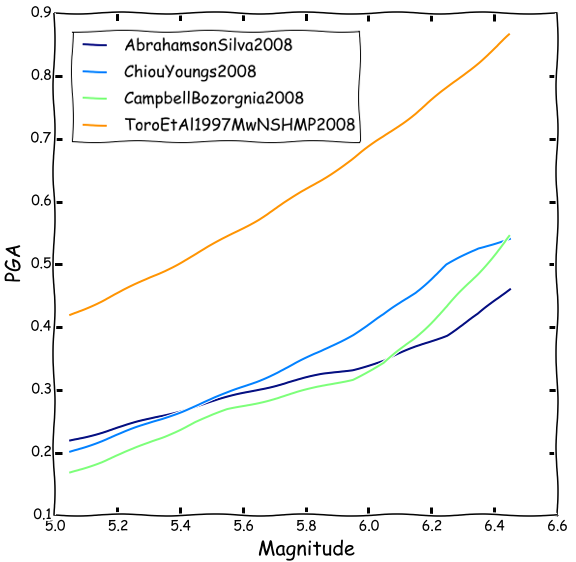
\includegraphics[width=1.0\textwidth]{gmpe_magnitude} 
		\caption{Variação da intensidade \gls{pga} com a magnitude.}
		\label{fig:gmpe_magnitude} 
	\end{subfigure}
	\quad
	\begin{subfigure}[t]{0.47\textwidth}
		\centering
		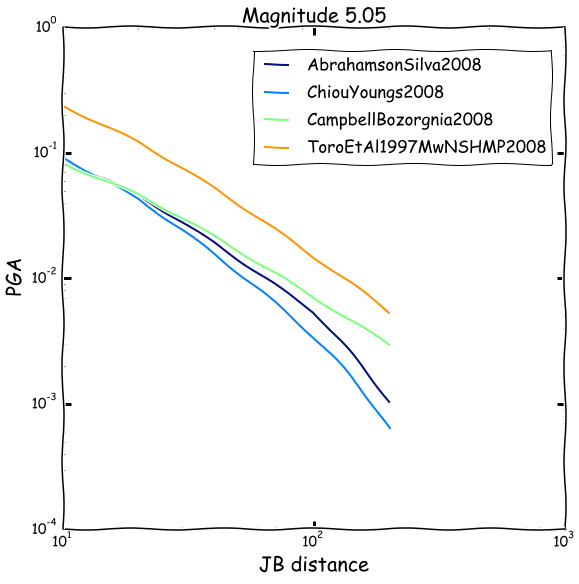
\includegraphics[width=1.0\textwidth]{gmpe_distance} 
		\caption{Variação da intensidade \gls{pga}) com a distância de Joyner-Boore.
		  para um valor de magnitude de 5.05 }
		\label{fig:gmpe_distance} 
	\end{subfigure}
	\caption{Variação das intensidades com a magnitude e distância, para diferentes GMPEs}
	\label{fig:gmpe} 
\end{figure}

A distância de \citet{joyner_1981} é uma das várias medidas de distância utilizadas e corresponde especificamente à
menor distância entre o local de avaliação da ameaça $S$ à projeção da ruptura na superfície da topografia. 

Apenas como exemplo, a forma funcional que \citet{toro_1997} dão à GMPE é

\begin{equation}
\begin{array}{lcl}
\ln I(M, R_M, \theta) 
&=& \theta_1 + \theta_2(M-6) + \theta_3(M-6)^2  \\
& & - \theta_4\ln (R_M) -(\theta_5 - \theta_4)\max\left[ \ln\left( \frac{R_M}{100} \right), 0 \right] -\theta_6 R_M \\
& & + \varepsilon_e + \varepsilon_a, \\
\end{array}
\end{equation}
com 
$$
R_M =  \sqrt{ R_{jb}^2 + \theta_7^2 }
$$
onde $R_{jb}$ é a distância de Joyner-Boore, $M$ é a magnitude de momento,
$\theta_i$ são as componentes do vetor de coeficientes e $\varepsilon_e$ + $\varepsilon_a$
são as incertezas epistêmica e aleatória do modelo.

Nesse exemplo 
\begin{equation}
\begin{array}{lcl}
\overline{\ln I}(M, D, \theta) & = & \theta_1 + \theta_2(M-6) + \theta_3(M-6)^2  \\
& & - \theta_4\ln (R_M)
-(\theta_5 - \theta_4)\max\left[ \ln\left( R_M / 100 \right), 0 \right]
-\theta_6 R_M
\end{array}
\end{equation}
e 
\begin{equation}
	\sigma(M, D, \theta)=\varepsilon_e(M,D) + \varepsilon_a(M,D).
\end{equation}


\subsection{Combinação de Incertezas e Avaliação da Ameaça Sísmica}
\index{cálculo da ameaça}
\label{sec:hazard}

A distribuição do número de tremores $N_{t i}$, na zona $i$, na janela de tempo $t$, por Poisson,
é dada por 
$$
P(N_{t i}=k)=e^{-\lambda_i t} \frac{(\lambda_i t)^k}{k!},\;k \in \mathbb{N},
$$
onde a taxa $\lambda_i$ representa o número médio de tremores na zona
$i$ por unidade de tempo, por exemplo, por ano.

Fixado um valor de intensidade $I$, o evento
\begin{equation} \label{formulapi}
\begin{array}{lll}
E(I, S, i)  & =  & \{ \mbox{Um tremor da zona }i \mbox{ gera uma intensidade} \\
&  &  \;\;\mbox{maior ou igual a} I \mbox{ em }S \}
\end{array}
\end{equation}
tem probabilidade $p_i=P \left\{ E(I, S, i)\right\}$.

Para cada tremor na zona $i$, o evento $E(I, S, i)$ ocorre, ou não.
Como resultado, é possível definir dois novos processos de contagem
em cada zona $i$: o processo $\tilde N_{t i}$, contando os tremores que 
causam intensidade maior ou igual a $I$ em $S$ e os que causam intensidade menor que $I$ em $S$.

\begin{figure}[H]
	\centering
	\begin{tabular}{l}
	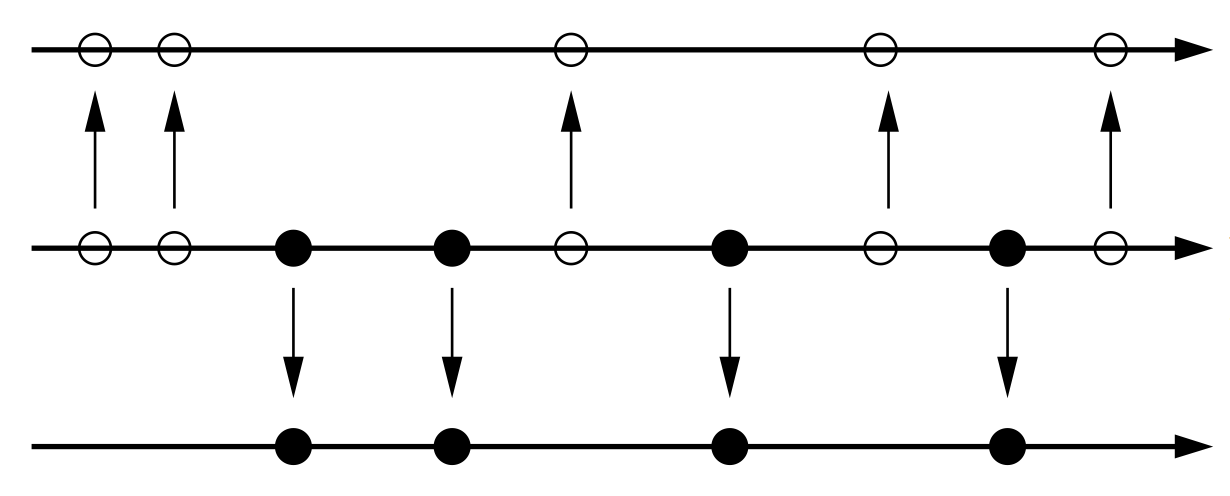
\includegraphics[width=0.80\textwidth]{poisson}
	\end{tabular}
	\caption{Separação do processo de chegada dos tremores da zona $i$ 
	em um processo causando, em $S$, intensidade maior que $I$ (bolas pretas) e intensidade 
	menor ou igual a $I$ (bolas brancas).}
\label{fig:poisson}
\end{figure}

É preciso utilizar o seguinte
\begin{lemma}
Considere um processo de Poisson $N_t$ com taxa de ocorrência $\lambda$.
Assumindo que as chegadas são de dois tipos: tipo 1 com probabilidade $p$,
e tipo 2 com probabilidade  $1 - p$ e que elas são independentes, 
então o processo $\tilde N_t$ do tipo 1 é um proceso de Poisson com taxa
$\lambda p$.
\end{lemma}
\begin{proof} Para cada $k \in \mathbb{N}$, calcule
$$
\begin{array}{lll}
P\Big(\tilde N_{t} =k \Big) & = & \displaystyle \sum_{j=k}^{+\infty} P\Big(\tilde N_{t} =k | N_{t}
=j\Big)  P \Big( N_{t} =j  \Big)\;\;\;\mbox{[Teorema da Probabilidade Total]}\\
&=& \displaystyle \sum_{j=k}^{+\infty} C_j^k p^k (1-p)^{j-k} e^{-\lambda t} \frac{(\lambda t)^j}{j!} \\
&=&e^{-\lambda t} \frac{(\lambda p t)^k}{k!} \displaystyle \sum_{j=0}^{+\infty} \frac{[\lambda (1-p)]^{j}}{j!} = e^{-\lambda p t} \frac{(\lambda p t)^k}{k!},
\end{array}
$$
o que mostra que $\tilde N_{t}$, usando a independência dos tipos de chegada em
intervalos disjuntos, é uma \gls{va} de Poisson com parâmetro
$\lambda p t$.\hfill
\end{proof}

Esse lema mostra que o processo $(\tilde N_{t i})_t$ é um processo de Poisson com taxa $\lambda_i p_i$.

Sendo $\mathcal{N}$ o número de zonas sísmicas, segue que a probabilidade de que haja $k$ sismos causando
intensidade maior que $I$ em $S$ na janela de tempo $t$ é
$$
\displaystyle
\begin{array}{lll}
P\Big(\displaystyle \sum_{i=1}^{\mathcal{N}} \tilde N_{t i} = k\Big)
&= &\displaystyle \sum_{x_1+\ldots +x_{\mathcal{N}}=k} P\Big(\tilde N_{t 1} = x_1; \ldots; \tilde N_{t \mathcal{N}} = x_{\mathcal{N}} \Big)\\
&= &\displaystyle{\sum_{x_1+\ldots +x_{\mathcal{N}}=k} \prod_{i=1}^{\mathcal{N}}}P\Big(\tilde N_{t i} = x_i \Big)\\
&= &\displaystyle \sum_{x_1+\ldots +x_{\mathcal{N}}=k} \prod_{i=1}^{\mathcal{N}} e^{-\lambda_i p_i t} \frac{(\lambda_i p_i t)^{x_i}}{x_{i}!}
\end{array}
$$
em que para a segunda igualdade foi utilizada a independência de  ${\tilde N}_{t 1}, \ldots, {\tilde N}_{t
\mathcal{N}}$.


Para $k=0$ na relação acima obtêm-se que
\begin{equation} \label{probinterest}
1-P( E_t(I, S) )= P(\overline{E_t(I, S)})=e^{-(\sum_{i=1}^{\mathcal{N}} \lambda_i p_i) t}.
\end{equation}

Com $\tilde N_t=\sum_{i=1}^{\mathcal{N}} \tilde N_{t i}$,
o valor esperado $\tilde N_t$ é o número médio de tremores causando intensidade maior que $I$ em $S$
 nos próximos $t$ anos e pode ser espresso por
\begin{equation} \label{formlambdatA}
\lambda_t(I, S)=\mathbb{E}\Big[ \tilde N_t \Big] =\sum_{i=1}^{\mathcal{N}} \mathbb{E}\Big[ \tilde N_{t i}\Big] =
\left( \sum_{i=1}^{\mathcal{N}} \lambda_i p_i \right) t.
\end{equation}

Usando essa relação e a equação \eqref{probinterest}, a probabilidade do evento $E_t(I, S)$
pode ser reescrita
\begin{equation}
P \left\{   E_t(I, S) \right\} =1-e^{-\lambda_t(I, S)}
\end{equation}
com $\lambda_t(I, S)$ dado por \eqref{formlambdatA}.


\subsubsection{Combinando todos os elementos}

Assumindo que as variáveis aleatórias da distância $D_i$ entre o tremor na zona $i$ e o local $S$ e magnitude $M_i$
são independentes e usando o Teorema da Probabilidade Total, obtém-se que
\begin{equation} 
p_i= \displaystyle \int_{m_i =M_{\min}(i)}^{M_{\max}(i)}
\int_{x_i =0}^{\infty}  P \left\{ \mbox{\small intensidade \normalsize }>I| M_i = m_i; D_i = x_i \right\}f_{M_i}(m_i) f_{D_i}( x_i )
\mathrm{d}m_i \mathrm{d}x_i
\end{equation}
onde $P \left\{ \mbox{\small intensidade \normalsize }>I| M_i = m_i; D_i = x_i \right\}$ 
é dada pelo de predição do movimento do chão \eqref{pgamodel}.

Para implementação, a integral acima é geralmente estimada discretizando as distribuições contínuas de 
magnitude $M_i, i=1,\ldots, \mathcal{N}$, e distância $D_i, i=1,\ldots, \mathcal{N}$.

